
\begin{figure}[H]
    \centering
    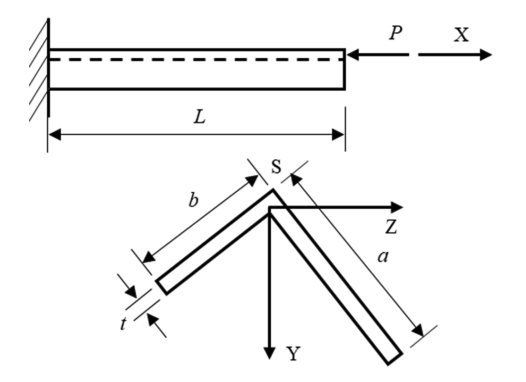
\includegraphics[width=0.4\linewidth]{Examples/frame-1030/img/frame-1030.png}
    \caption{Caption}
    \label{fig:1030-setup}
\end{figure}

\subparagraph{Context}
\cite{du2021threedimensional} and \cite{alsafadie2010corotational}.


\FrameSection{
label/problem=frame-1030,
label/section=a,
%
shape=Angle,
kinematics/section={\eqref{eq:wagner-gl-strain-pi}},
% Label
E=193.05,
nu=0.3,
unit/length={\milli\meter},
unit/stress={\giga\pascal}
}

\subparagraph{Results.}
Load–deflection curves at the tip \(\reflenx=L\) are plotted in \cref{fig:1030-soln}. 

\begin{figure}[H]
    \centering
    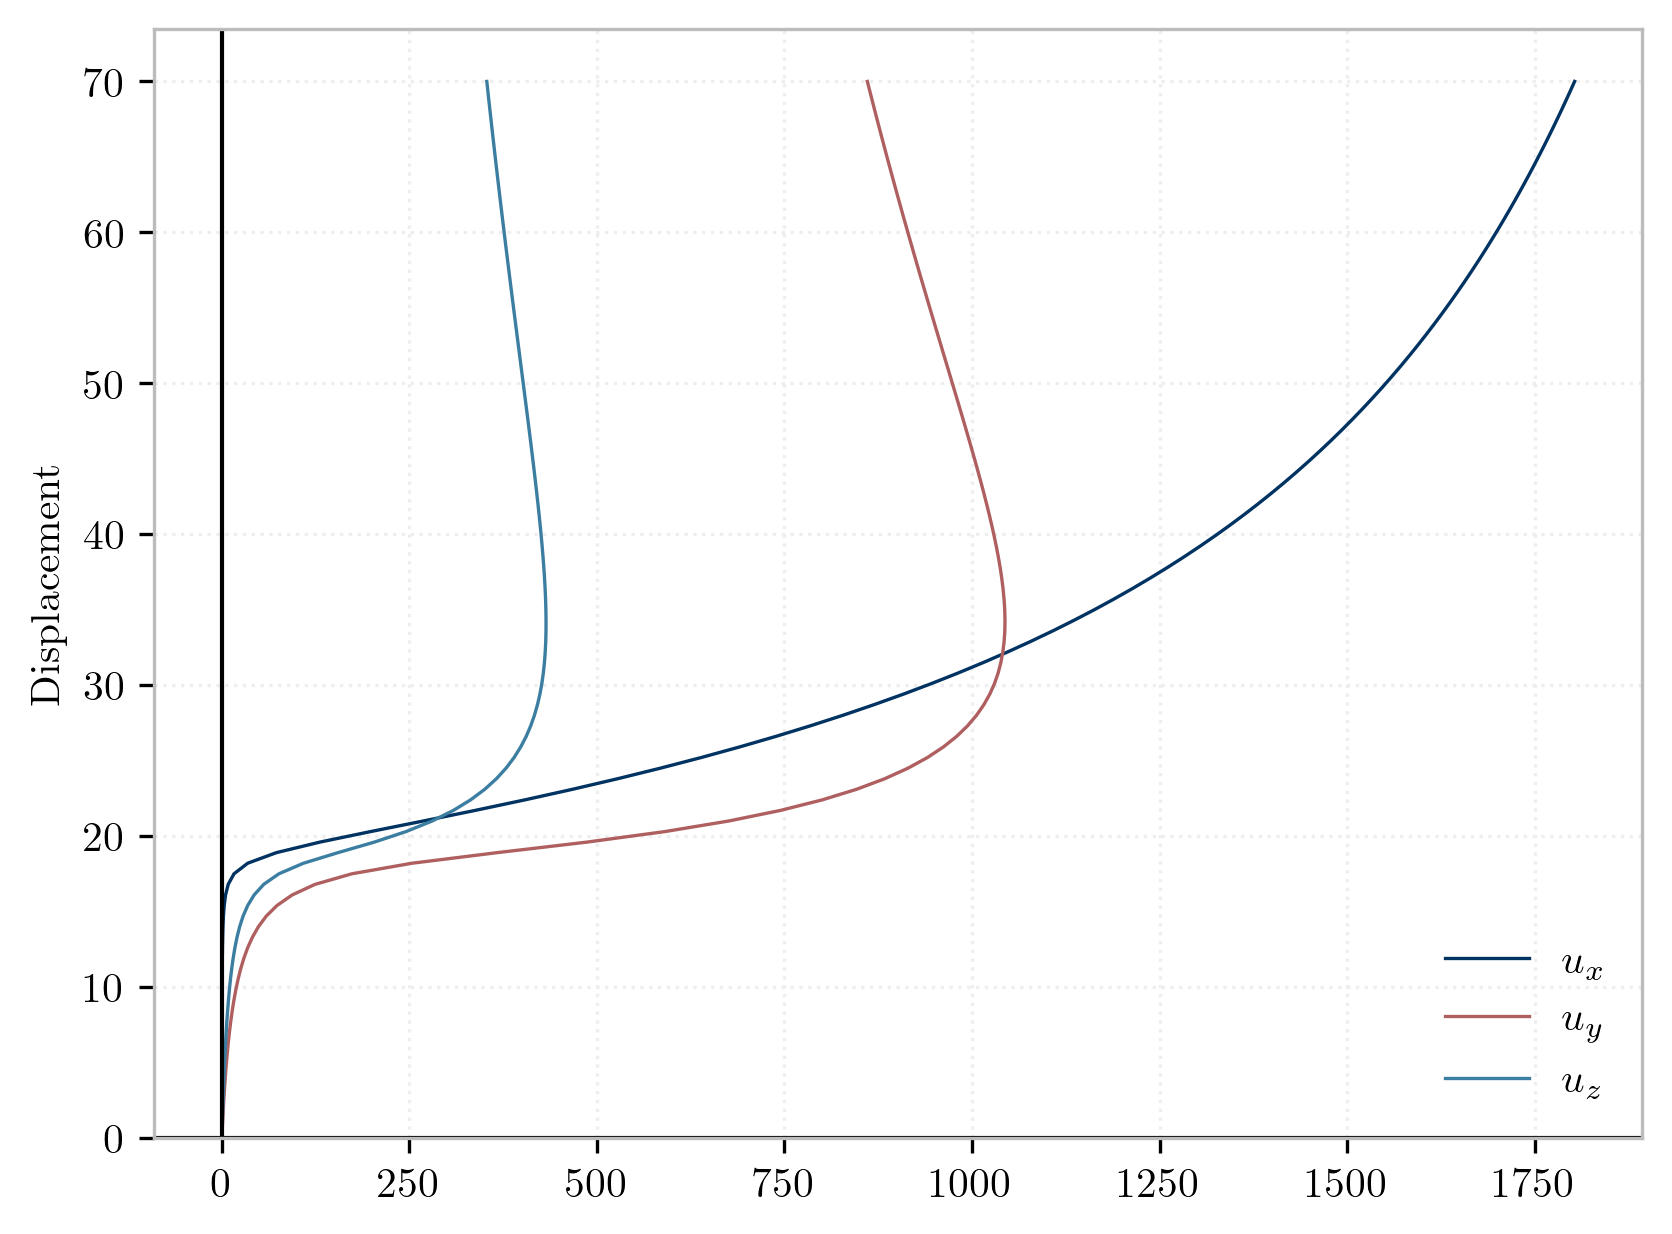
\includegraphics[width=0.45\linewidth]{Examples/frame-1030/img/1030-soln.png}
    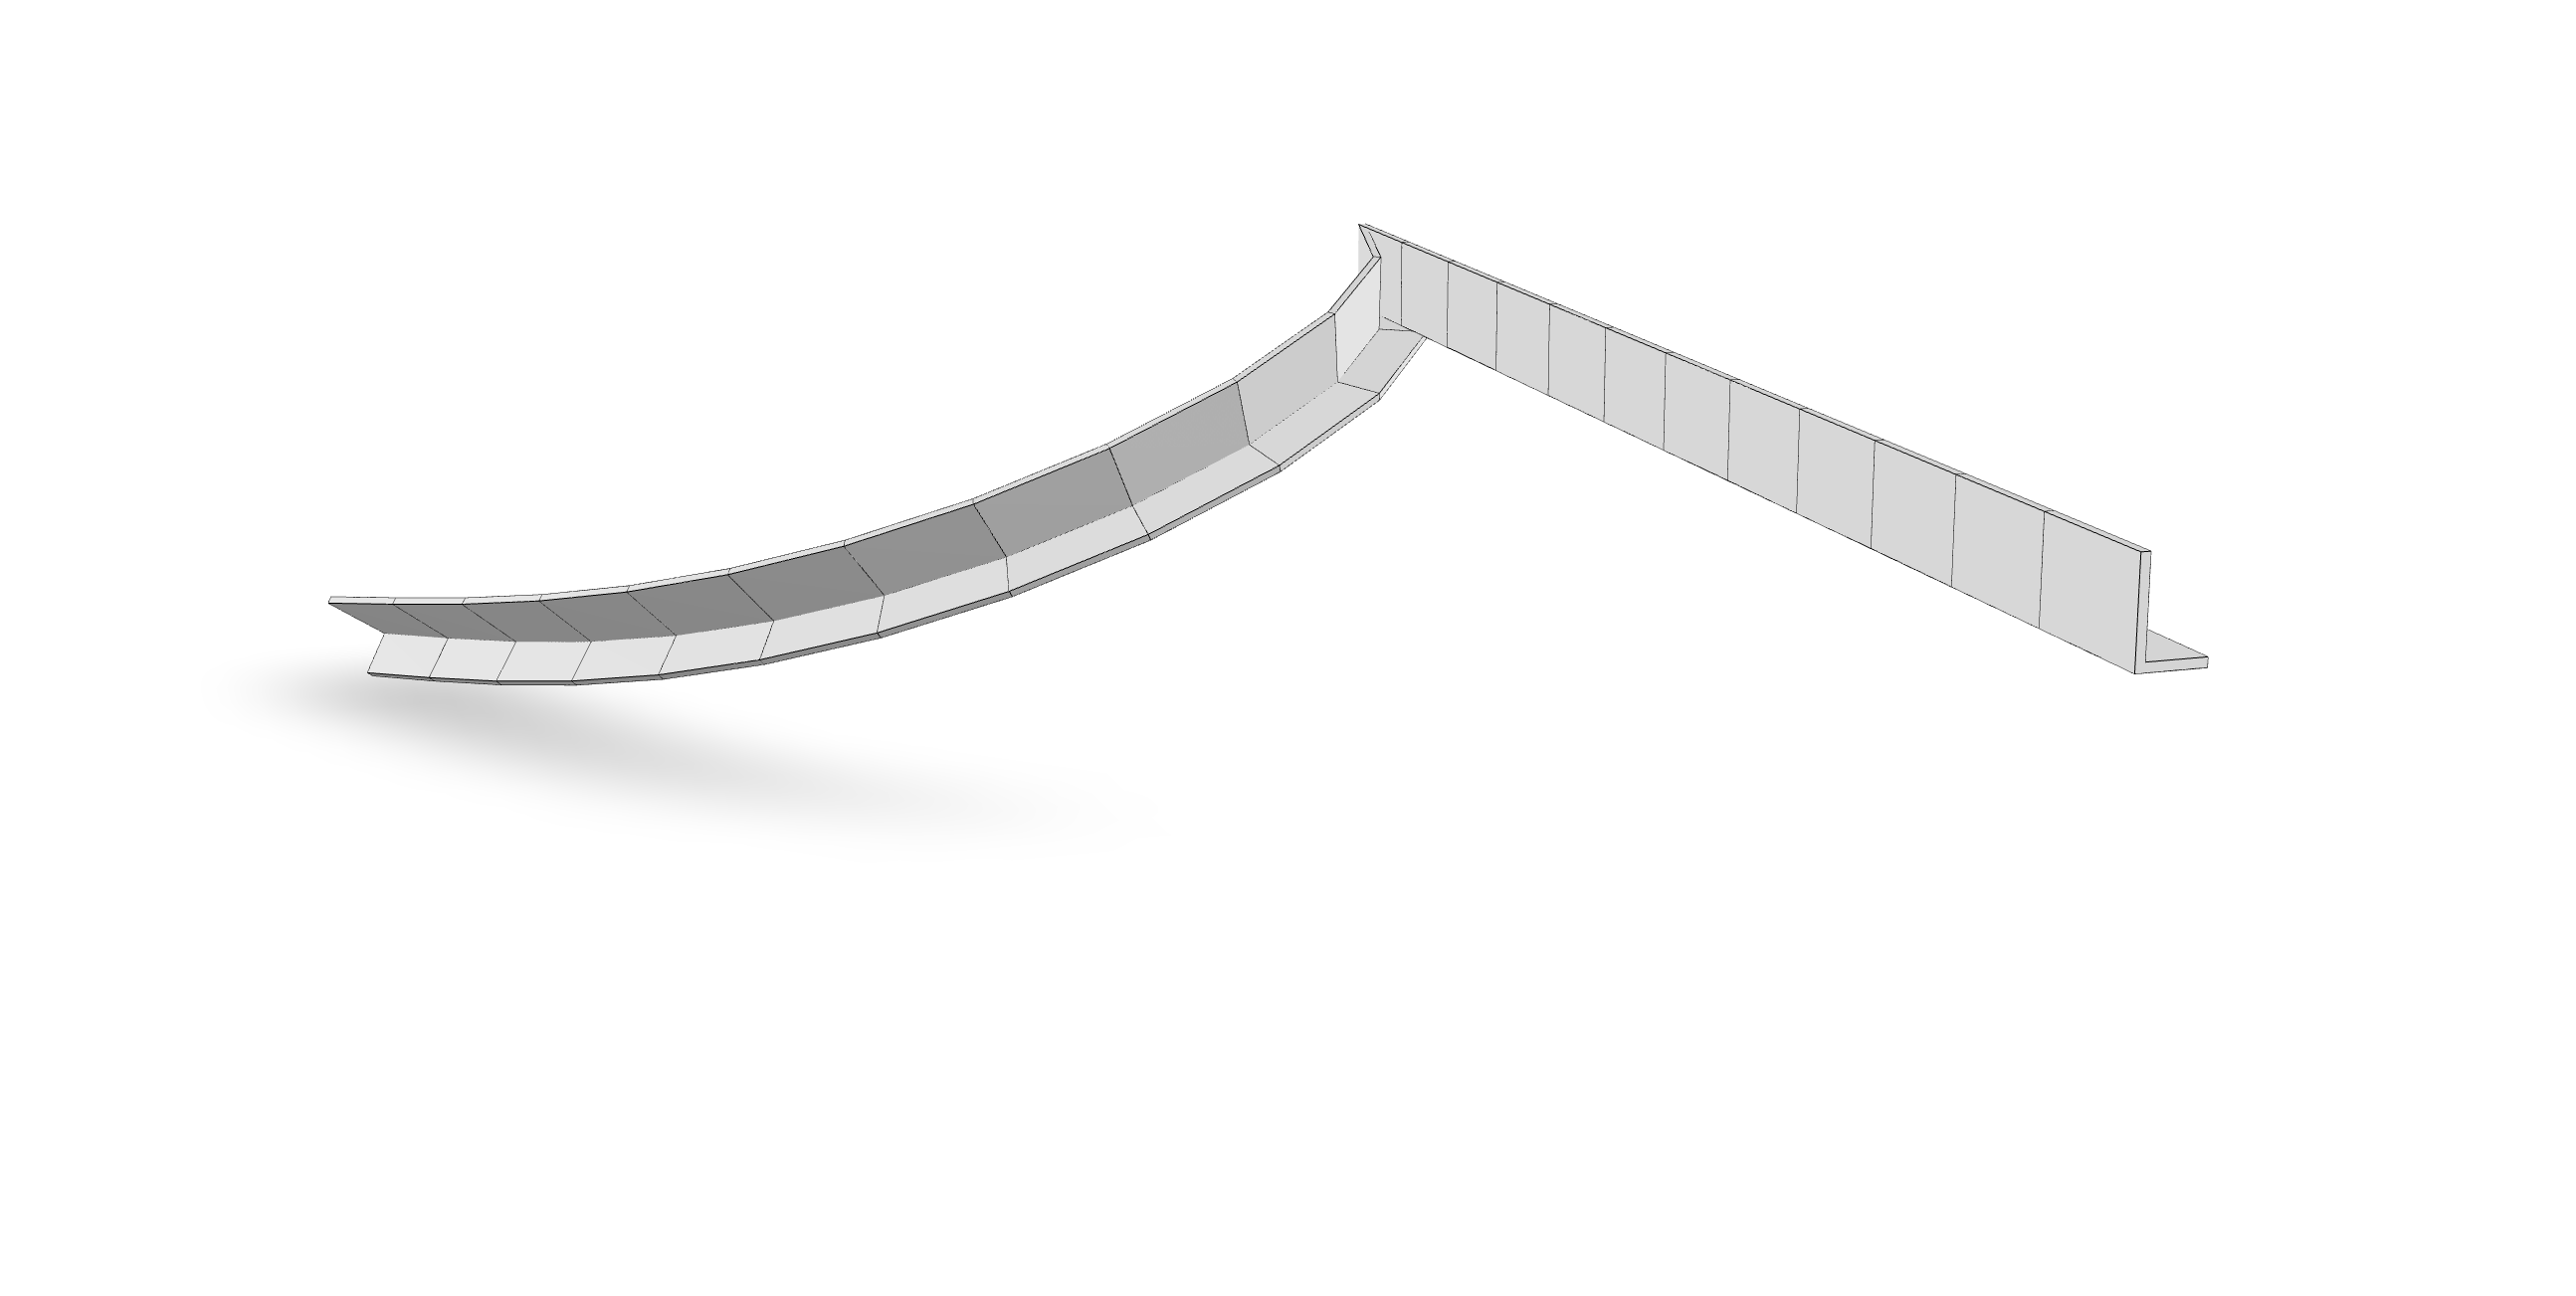
\includegraphics[width=0.5\linewidth]{Examples/frame-1030/img/1030-render.png}
    \caption{Tip displacements for Example~\ref{sec:frame-1030} with 4 \ExactFrame{I} elements.}
    \label{fig:1030-soln}
\end{figure}